\documentclass[b5paper]{standalone}
\usepackage{fontspec}
\usepackage{polyglossia}
\usepackage{tikz}
\usepackage{pgfplots}
\usepackage{ifthen}   
\usepackage{amsmath}
\usepackage{siunitx}
\usetikzlibrary{calc}
%
\setmainlanguage{english}
\setotherlanguages{arabic}
\newfontfamily\arabicfont[Scale=1.0,Script=Arabic]{Scheherazade}
\newfontfamily\urdufont[Scale=1.0,Script=Arabic]{XB Tabriz}

%---------------

\begin{document}
\begin{urdufont}

\begin{tikzpicture}
%BHloop
\begin{scope}[xshift=6cm]
\draw (0,0) node {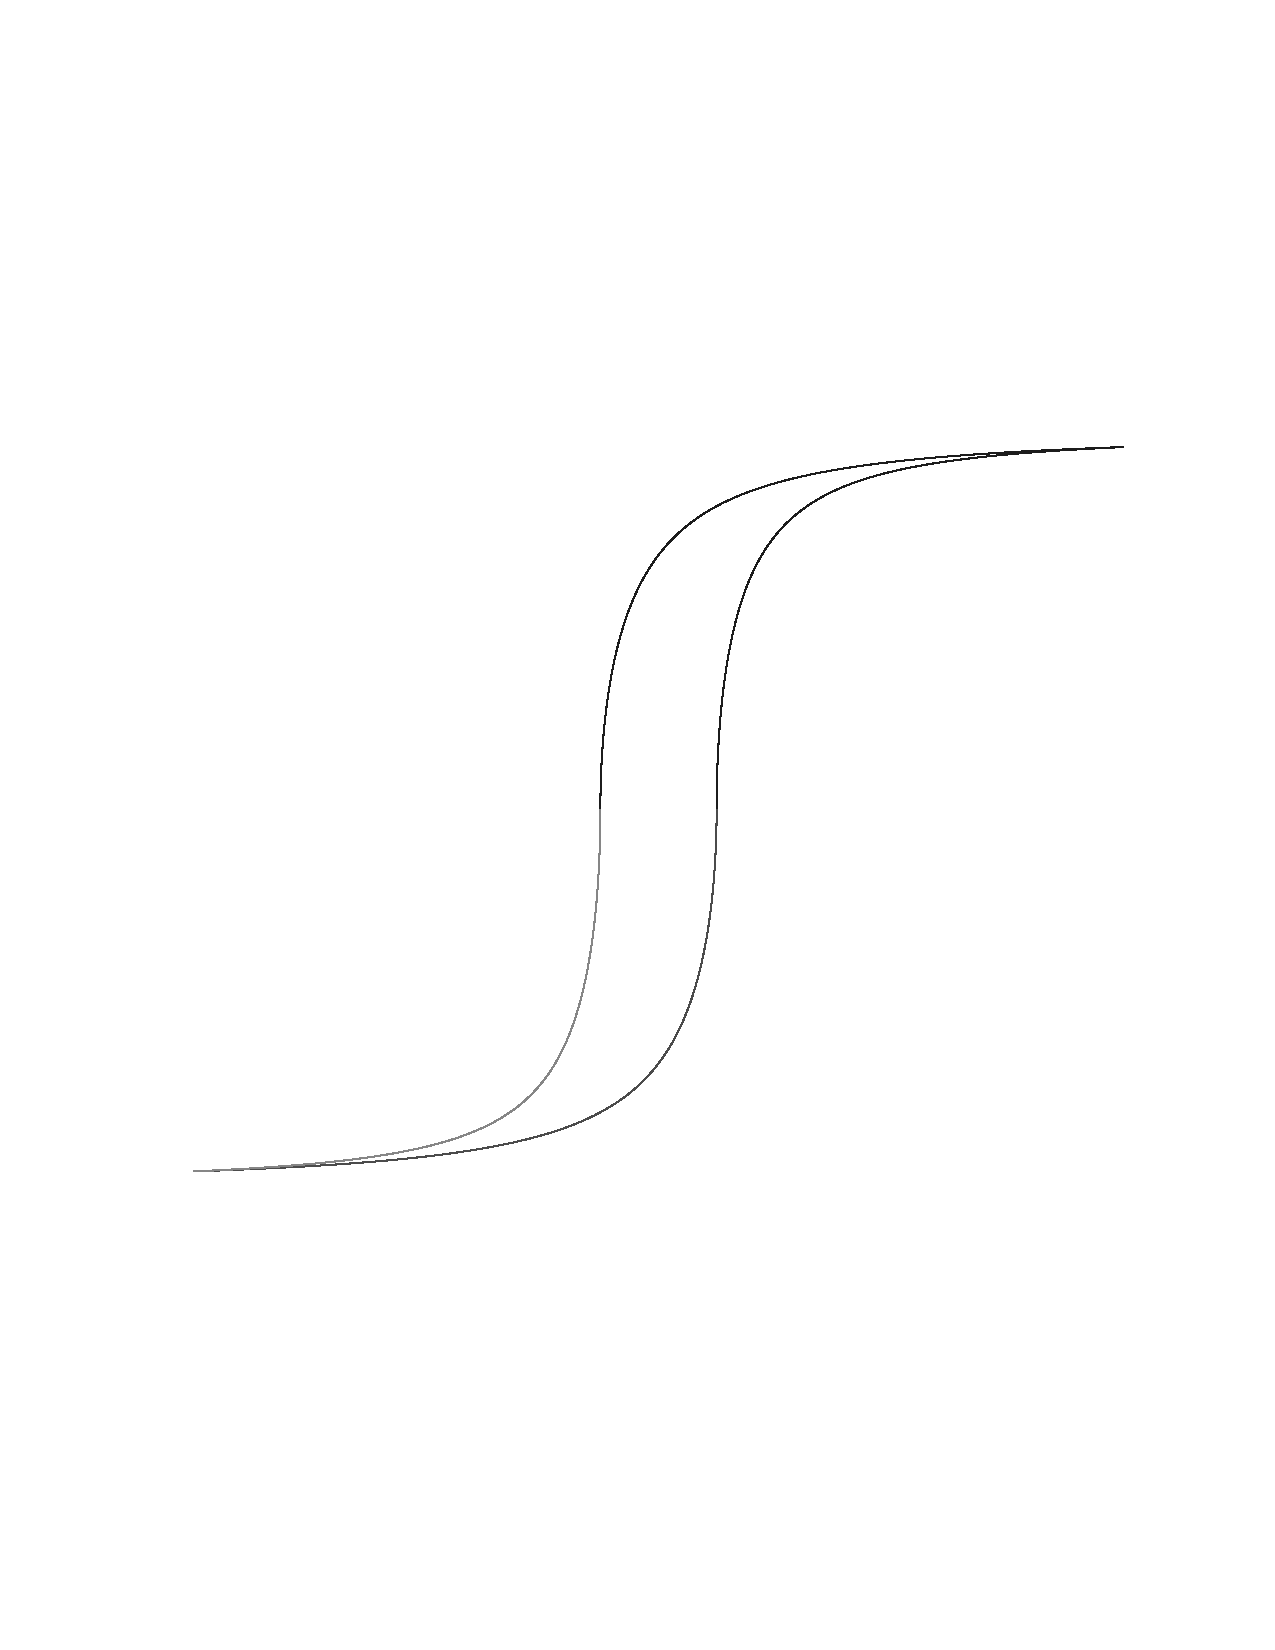
\includegraphics[width=0.5\linewidth]{ExcitationCurrentBHloopOnly.pdf}};
\draw(-2.2,0)--(2.2,0);
\end{scope}
%excitation current
\begin{scope}
\draw (0,0) node {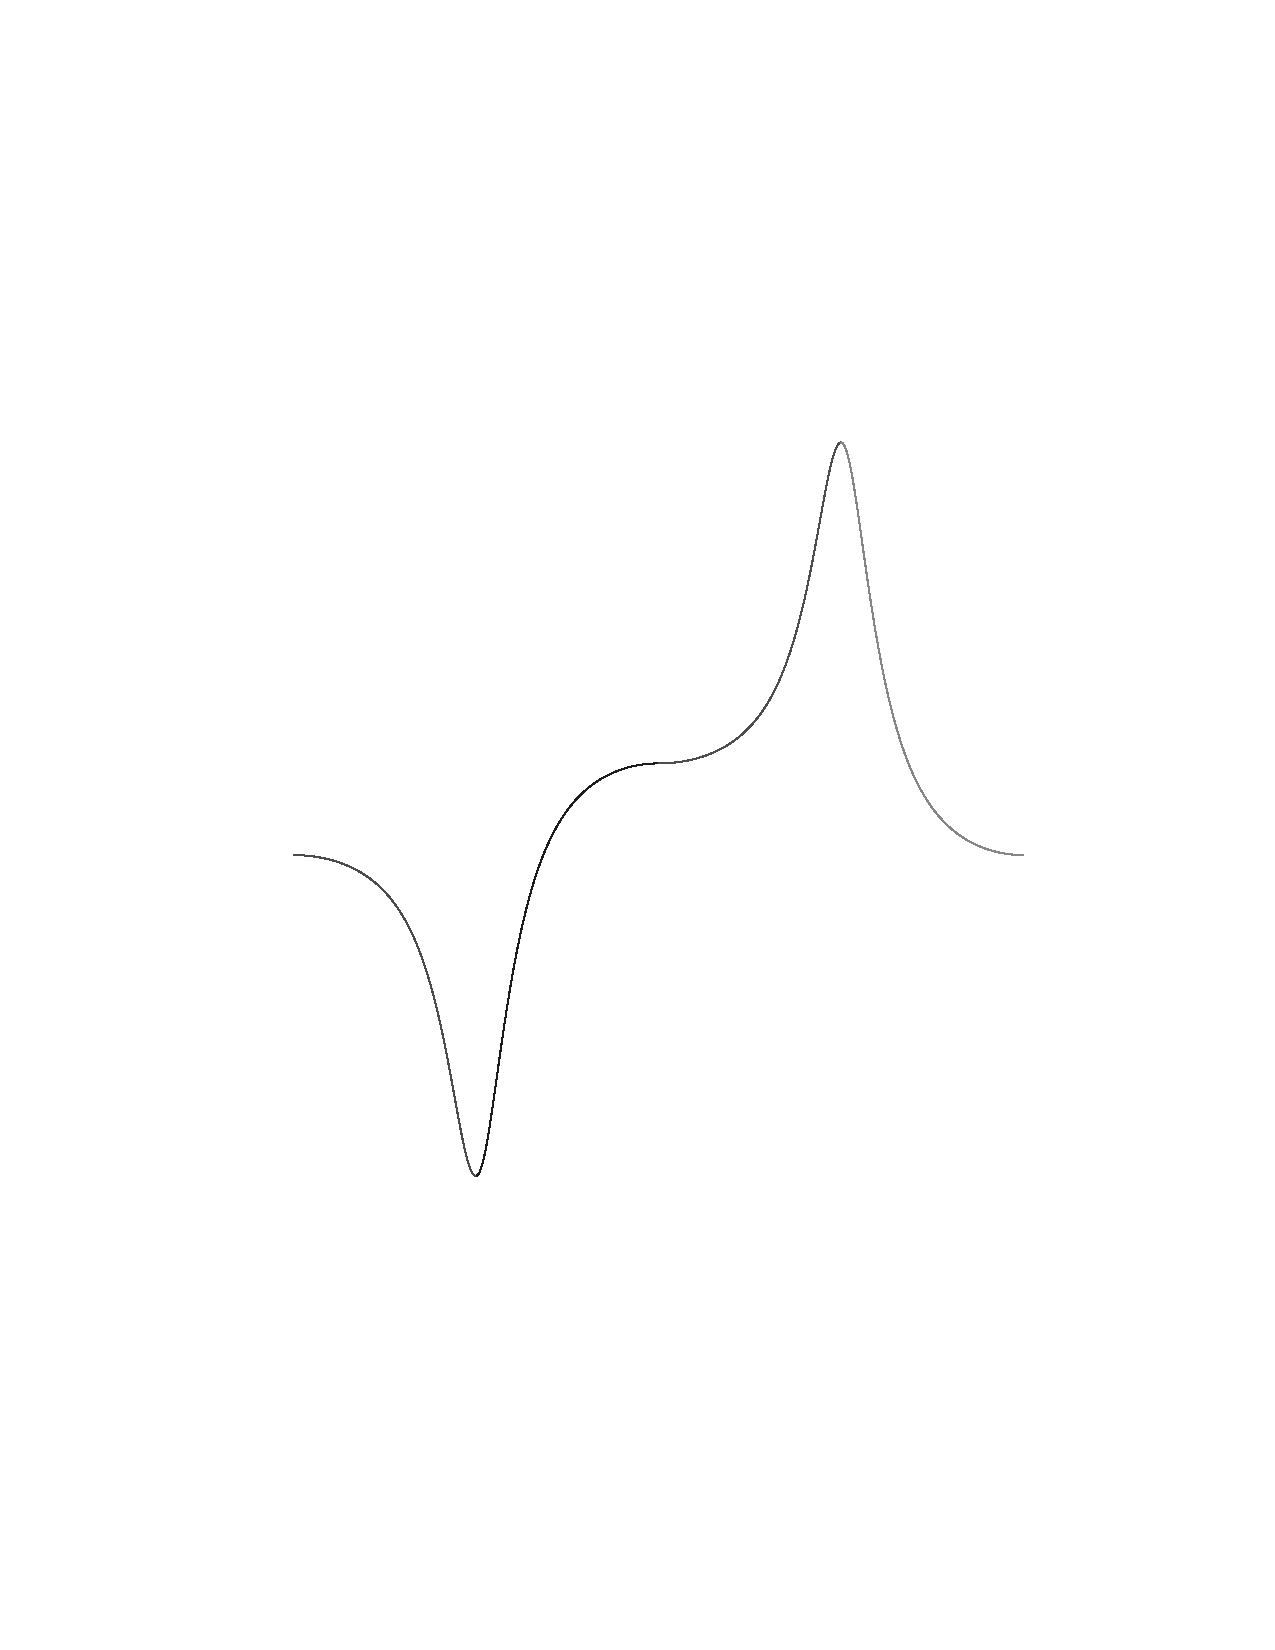
\includegraphics[width=0.5\linewidth]{ExcitationCurrent.pdf}};
\end{scope}
\draw(-2,0)--(2,0);
%axis

\end{tikzpicture}
\end{urdufont}
\end{document}

